\section{Introducción}
Definitivamente {\LaTeX} es una gran herramienta de trabajo para documentos profesionales, la gran cantidad de información libre y disponibilidad de herramientas cada vez más sofisticadas hace que sea el favorito de estudiantes y profesionales en todas las ramas.

En este pequeño tutorial introductorio se abordará los aspectos de instalación, configuración y compilación de este \verb|Template|, y la descripción de los formatos nuevos introducidos desde la versión 1.7. 

Naturalmente encontrarás errores así que no dudes en escribir a \url{prlomarconi@gmail.com}, gracias.

\section{Instalación y Configuración del Compilador y Editor de Texto}
En este punto imagino que conoces lo básico de {\LaTeX} para compilar rápidamente este \verb|Template|; de seguro ya tienes un 'Compilador\&Editor de Texto' instalado, sin embargo, te recomiendo que no saltes esta parte porque talvez exista un paso importante que luego omitas y cause error de compilación.

\subsection{Compilador: Miktex (Windows) o TexLive (Windows/Linux)}
Ambos son \verb|open-source| y pesan entre 160Mb y 3.4Gb respectivamente, contienen todos los paquetes \verb|(packages)| que se usan para cualquier tipo de documento, pero solo se debe escoger uno, para este \verb|Template| se usó \verb|Miktex| sobre \verb|Windows10 x64|, porque pesa menos que \verb|TexLive| y ofrece la ventaja de instalación de paquetes \verb|On the Fly|, pero puedes usar \verb|TexLive| si usas \verb|Linux| y así compartir tus experiencias, en general no debería existir problemas de compilación para ambos casos.

Es recomendable descargar la última \href{http://miktex.org/download}{versión} de \verb|Miktex|, después de finalizada la instalación se debe actualizar con \verb|Update(Admin)| todos los paquetes fig. \ref{fig:Miktex}(a), normalmente existirán actualizaciones cuando se instala por primera vez pero eventualmente no se pedirán más.

Lo siguiente es elegir formato de hoja(\verb|Letter(letterSize)|), refrescar la base de datos (\verb|Refresh FNDB|), actualizar formatos (\verb|Update Formats|) y elegir instalación de paquetes (\verb|On the Fly|) fig. \ref{fig:Miktex}(b), este último permite instalar automáticamente paquetes faltantes de este \verb|Template| pero requiere \verb|Texworks|, sobre esto se comentará después. 

\begin{figure}[H]
	\centering
	\subfigure[Paso 1]{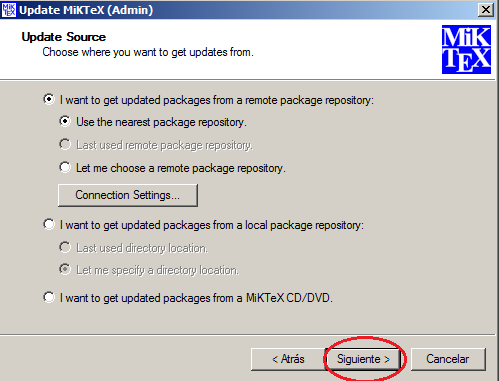
\includegraphics[width=0.4\linewidth]{Figures/Miktex1}}
	\subfigure[Paso 2]{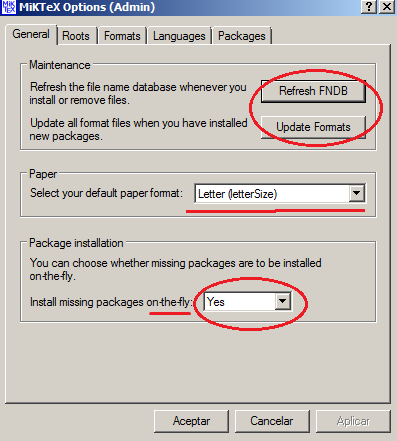
\includegraphics[width=0.4\linewidth]{Figures/Miktex2}}
	\caption{Pasos MikTex}
	\label{fig:Miktex}
\end{figure}

\subsection{Editor de Texto: TeXstudio}
\href{http://texstudio.sourceforge.net/}{TeXstudio} es un potente \textbf{Editor de Texto(Windows/Linux)} para todo tipo de usuarios, viene con traducción al español, es de fácil configuración y se integra muy bien con \verb|Miktex|.(Si deseas usar un editor diferente puedes elegir alguno de la tabla \href{http://en.wikipedia.org/wiki/Comparison_of_TeX_editors}{online} comparativa.)  

Después de la instalación se realiza unas configuraciones básicas:

\Activate
\begin{easylist}[itemize]
	& Por defecto \verb|TeXstudio| viene con el diccionario (\verb|spelling/hyphen/thesaurus| - ortografía/separación/sinónimos) en \verb|inglés|, para agregar \verb|español| se debe descargar la última \href{http://extensions.openoffice.org/de/project/spanish-espanol}{versión} de \verb|OpenOffice/Extensions|, también puedes descargar el diccionario  \href{http://extensions.openoffice.org/de/project/english-dictionaries-apache-openoffice}{inglés}. Lo mas probable es que descargues un archivo sin extensión, debes renombrarlo a \verb|.zip| y a \verb|.oxt| además de descomprimirlo, debe quedar como en la fig. \ref{fig:TeXstudio}(a).	
	& Después de iniciar \verb|TeXstudio|, vas a \verb|Options/General| e importas los diccionarios \textbf{(Import Dictionary)} que acabas de descargar, también importas \verb|Thesaurus| y si deseas escoges el idioma de la interfaz fig. \ref{fig:TeXstudio}(b). Para terminar vas a \verb|Grammar| y direccionas el directorio de palabras \verb|WordsDirectory|, puedes usar solo la carpeta \verb|es_ANY| o lo dejas como en la fig. \ref{fig:TeXstudio}(c), para español e inglés.
\end{easylist}
\Deactivate

\begin{figure}[H]
	\centering
	\subfigure[Paso 1]{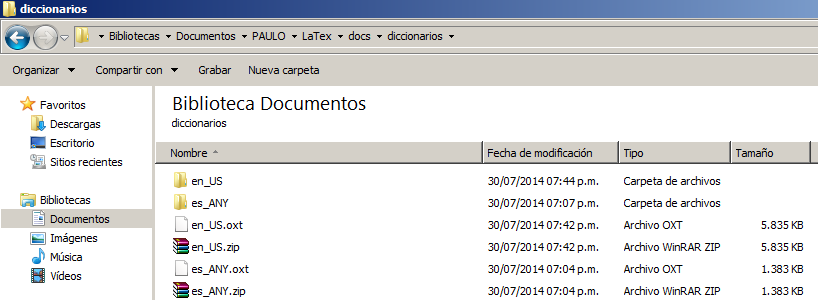
\includegraphics[width=0.45\linewidth]{Figures/TeXstudio1}}
	\subfigure[Paso 2]{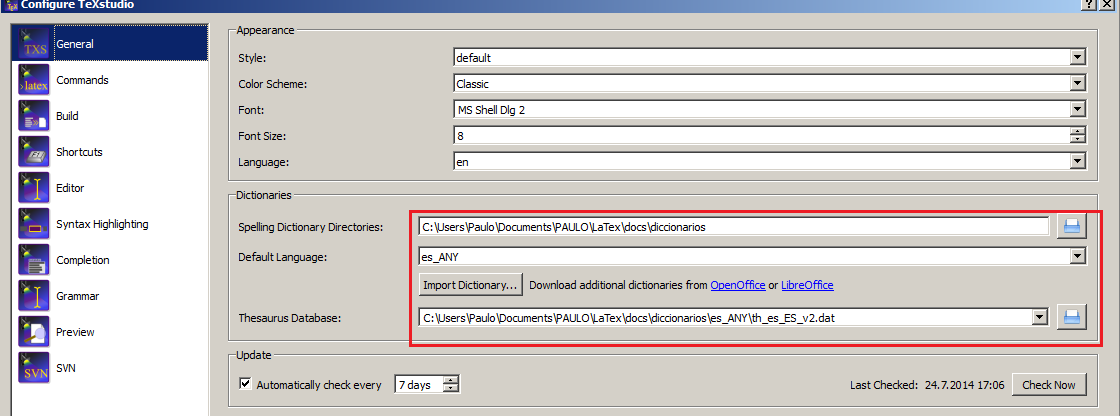
\includegraphics[width=0.45\linewidth]{Figures/TeXstudio2}}
	\subfigure[Paso 3]{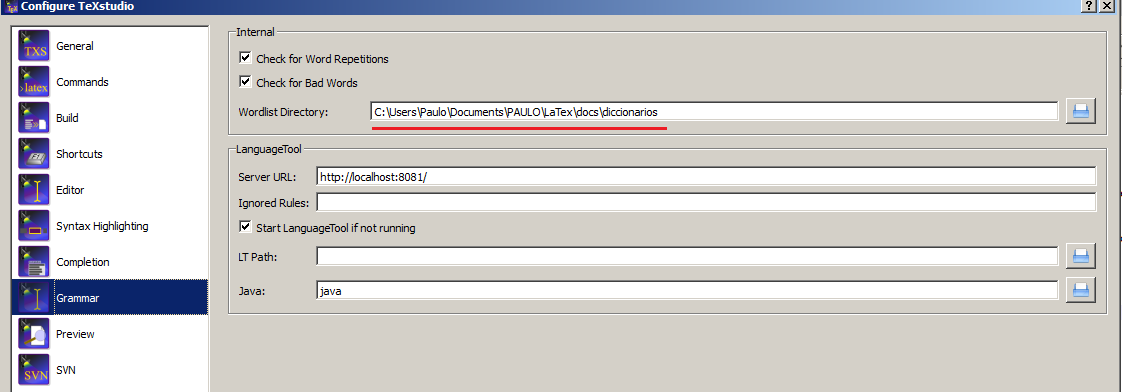
\includegraphics[width=0.45\linewidth]{Figures/TeXstudio3}}
	\caption{TeXstudio, pasos de configuración.}
	\label{fig:TeXstudio}
\end{figure}

		
Por último, es recomendable instalar \href{http://www.perl.org/get.html}{Strawberry Perl} para utilizar herramientas extras como \textsf{Glossary F10}, \verb|Bibliography F11|, \verb|Index F12| y \verb|pax|

\subsubsection{Crear Macros}
\verb|TeXstudio| ofrece la posibilidad de agregar \verb|macros| de uso frecuente; por ejemplo, \verb|easylist| para enlistar y \verb|\verb||| para imprimir texto \verb|raw|.
\begin{lstlisting}[language=tex, caption=, label={}]
\Activate
\begin{easylist}[itemize]	
	& 	
\end{easylist}
\Deactivate
\end{lstlisting}
Crear un \verb|macro| es fácil, se va a \verb|Macros/editmacros| y se agrega según las fig. \ref{fig:TeXstudioMacros}, ahora ambos tienen un nuevo \textit{hotkey}. 

\begin{figure}[H]
	\centering
	\subfigure[Paso 1]{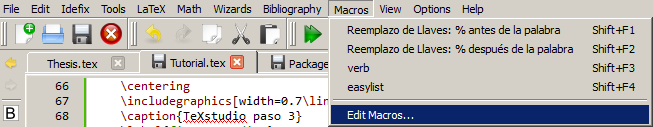
\includegraphics[width=0.6\linewidth]{Figures/TeXstudio4}}
	\subfigure[Paso 2]{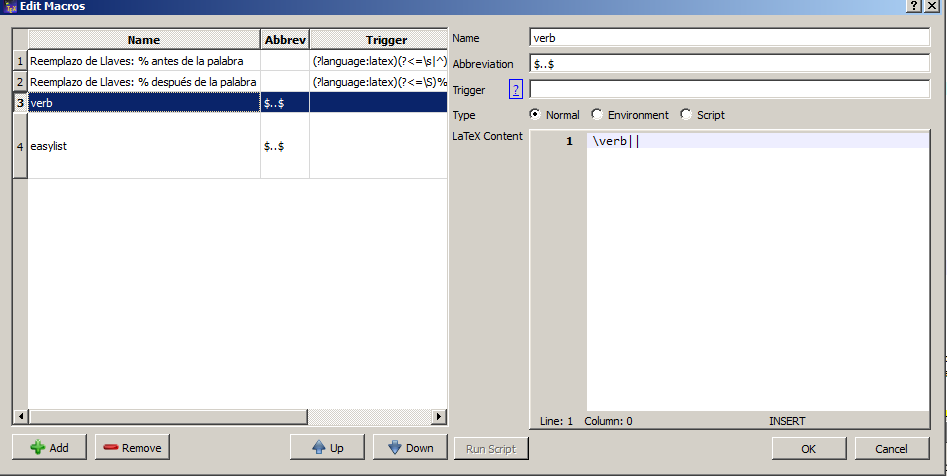
\includegraphics[width=0.47\linewidth]{Figures/TeXstudio5}}
	\subfigure[Paso 3]{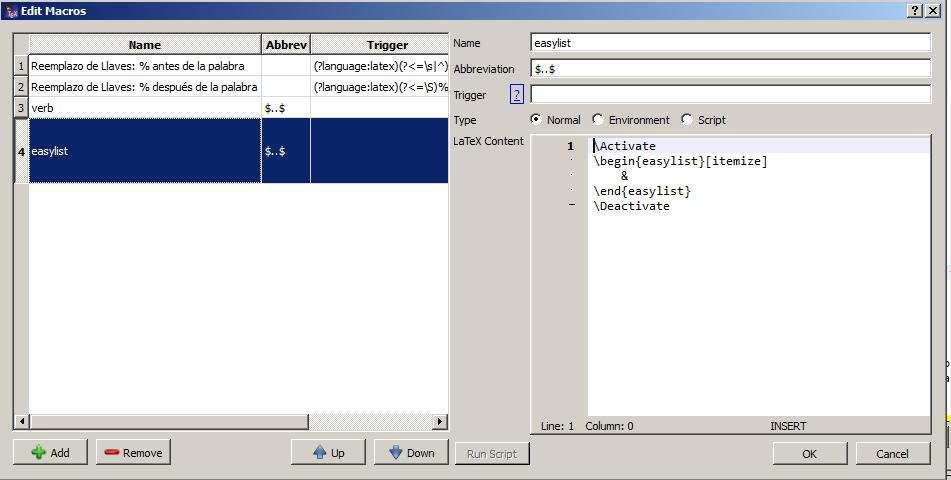
\includegraphics[width=0.47\linewidth]{Figures/TeXstudio6}}
	\caption{TeXstudio, creación de macros}
	\label{fig:TeXstudioMacros}
\end{figure}
	
\section{Estructura y distribución de los formatos}
Desde la versión 1.7 se agregaron dos nuevos formatos; \verb|Journal IEA| y \verb|Artículo IEA|; desarrollados para el Instituto de Electrónica Aplicada (IEA) de la Facultad de Ingeniería de la Universidad Mayor de San Andrés (UMSA), La Paz - Bolivia.

Por tanto, este nuevo template está organizado de la siguiente forma:
\Activate
\begin{easylist}[itemize]
	& \textmyfont{Thesis}: formato para la realización del Proyecto de Grado o Tesis.
	& \textmyfont{Profile}: formato del Perfil de Proyecto de Grado.
	& \textmyfont{JournalIEA}: formato que une todos los Artículos a través del paquete \textmyfont{pdfpages}.	
	& \textmyfont{ArticlesIEA}: contiene los Artículos académicos para \textmyfont{JournalIEA}, distribuido en carpetas \textsf{Article1, Article2}. Para agregar cuantos Artículos se deseen basta clonar \textmyfont{Article1 o Article2} y renombrar su contenido.
	& \textmyfont{MainTutorial}: formato de este Tutorial.
	& \textmyfont{Tutorial}: contenido de este Tutorial.
	& \textmyfont{Preamble}: contiene \textmyfont{UMSAetn.cls} y \textmyfont{Administrative.sty}.
\end{easylist}
\Deactivate

Antes de abrir y compilar cualquier \textmyfont{formato.tex}, no está demás revisar la estructura siguiente:
\begin{lstlisting}[language=tex, caption={}, label={}]
% %----- Preámbulo------
\documentclass[oneside,letterpaper,10pt]{book}
\usepackage{package} .....
% %----- end Preámbulo---

% %----- Cuerpo ---------
\begin{document}
	content...
\end{document}
% %----- end Cuerpo-----
\end{lstlisting}

Son solo 2 partes, cualquier documento que se crea con {\LaTeX} tiene esta estructura; Preámbulo y Cuerpo.

\begin{quote}\label{quo:Importante}
	\textbf{Importante:} Los códigos que hacen referencia a los documentos \verb|.tex| y \verb|.sty| que tienen en el encabezado la palabra \textbf{(realimentado)}, hacen uso del comando \verb|\lstinputlisting{}|, lo que significa que cualquier cambio en alguno se reflejará en las '\textbf{referencias a código}' que tengan la palabra \textbf{(realimentado)}. 
	
	Puedes probar aumentando algunas lineas vaciás en el encabezado \verb|arara| de \textsf{MainTutorial.tex}, compilas y notarás los cambios en código \ref{cod:arara}, el motivo es para no tener código redundante en \verb|Tutorial.tex| y mantener actualizado algún cambio posterior, no afecta de ninguna manera a los resultados.
\end{quote}
 
\subsection{Instalación de paquetes faltantes}
Si tratas de compilar con \verb|Build&Compile F1|, el \verb|Log| de errores mostrará que faltan muchos paquetes, la opción obvia es ir a \verb|Miktex/PackageManager(Admin)| e instalar los paquetes uno a uno, eventualmente no mostrará mas errores, aun así \verb|TeXstudio| no compilará y mostrará un estado de \textit{standby} en el puntero del \textit{mouse}. 

Para resolver definitivamente la instalación de paquetes, abres un \verb|formato.tex|; por ejemplo \textsf{MainTutorial.tex}, con \verb|TeXworks| de \verb|Miktex|; que viene instalado por defecto, notarás que también es un editor de texto como \verb|TeXstudio| pero básico y simple, nuevamente intentas la compilación y automáticamente \verb|Miktex| hará uso de su herramienta \verb|On the Fly| para instalar los paquetes o estilos \verb|.sty| faltantes a través de Internet, después de un tiempo de descarga e instalación por fin verás que \verb|formato.tex| compiló satisfactoriamente con la creación de \verb|formato.pdf| en su carpeta respectiva.

\subsection{Primera compilación completa para cualquier formato}
Si revisas \verb|formato.pdf|; que acabas de compilar en el punto anterior, notarás que no tiene Bibliografía, Indice de Palabras, Glosario y Acrónimos, el motivo es que cada uno de ellos requiere un \verb|Build| independiente.

Es decir, en un documento simple como:
\begin{lstlisting}[language=tex, caption=, label={}]
\documentclass{report}

\begin{document}
	content...
\end{document}
\end{lstlisting}
solo se requiere compilar(\verb|Build: pdflatex|) con la tecla \verb|F1| una vez, pero en el caso de un libro o los formatos en este \verb|Template|; que necesitan de Bibliografía(\verb|Build: bibtex|), Indice de palabras(\textmyfont{Build: makeindex}) y hasta Glosarios/Acrónimos(\verb|Build: makeglossaries|), la tarea se convierte engorrosa. 

Pues verás, si deseas compilar todos los \verb|Builds| tendrías que:
\Activate
\begin{easylist}[itemize]	
	& Ir a \verb|Tools/Build&Compile F1| 
	& Luego \verb|Tools/Glossary F10| 
	& \verb|Tools/Bibliography F11|
	& \verb|Tools/Index F12| 
	& Nuevamente \verb|Tools/Build&Compile F1| para incluir Bibliografía, Indice de palabras y Glosario/Acrónimos. 
	& Una última vez \verb|Tools/Build&Compile F1| para evitar errores.
\end{easylist}
\Deactivate

Notas lo mecánicamente aburrido que puede ser si deseas ver como queda \verb|Tutorial.pdf| cada vez que lo necesites, pues es aquí donde \verb|arara| muestra todo su potencial al automatizar todas la compilaciones con una sola combinación de teclas. 

\href{https://github.com/cereda/arara}{Arara} es una aplicación/herramienta \verb|Java| de 'Automatización Controlada de Compilación', a través de directivas permite agregar los \verb|Builds| que cualquier \verb|formato.tex| necesita para finalmente compilar \textbf{TODO} de una sola vez.

Después de descargar e instalar \verb|arara|, debes agregar un nuevo comando según la fig. \ref{fig:arara1}, y lo encontrarás en \verb|Tools/User/1: Arara Alt+shift+F1|.

\begin{figure}
	\centering
	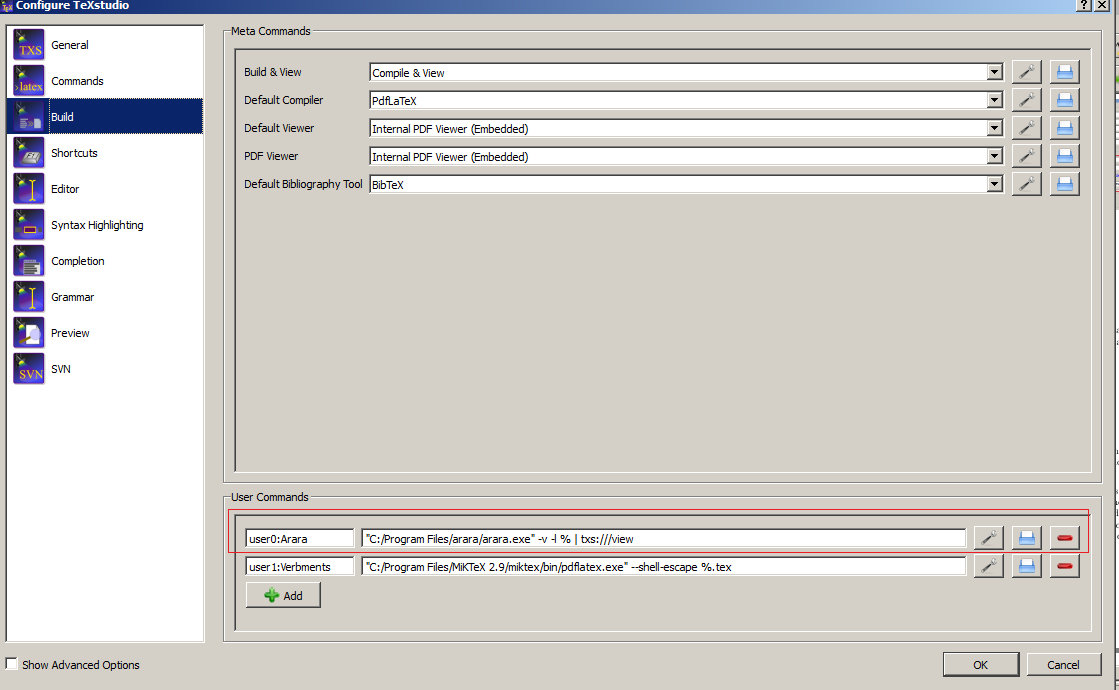
\includegraphics[width=0.7\linewidth]{Figures/arara1}
	\caption{configuración \textbf{arara}}
	\label{fig:arara1}
\end{figure} 

El encabezado \verb|arara| \ref{cod:arara} muestra los \verb|Builds| que usará en orden descendente, cuando ejecutas \textsf{Alt+shift+F1} verás en el \verb|Log| de \textmyfont{TeXstudio} como compila los \verb|Builds| uno a uno hasta finalizar todo el proceso. 
	
\lstinputlisting[language=tex, 
caption={MainTutorial.tex, arara (realimentado)}, 
label={cod:arara},
linerange={1-10}]{../Tutorial/MainTutorial.tex}
				
\section{Uso de estilos.sty}
A diferencia de un \verb|documento.tex| común, el \verb|estilo.sty| evita errores de anidamiento con \verb|loops| condicionales y se carga las veces que sea necesario, por eso se recomienda su uso en el Preámbulo; ref. \href{http://tex.stackexchange.com/questions/91167/why-use-sty-files}{why-use-sty-files}, y requiere conocimiento para crear \verb|packages|; ref. \href{http://www.sharelatex.com/learn/Writing_your_own_package}{Writing your own package}.

Un ejemplo simple de \verb|estilo.sty|:
\begin{lstlisting}[language=tex, caption=, label={}]
\ProvidesPackage{nombre} 
	code......
\endinput
\end{lstlisting}
y para invocarlo en el Preámbulo, \verb|\usepackage[opciones]{nombre}|.

\section{Preamble/UMSAetn.cls}
Contiene todos los paquetes y configuraciones básicas para todos los formatos usados en este \verb|Template|, a continuación se describirá que contiene cada sección de la clase.
\subsection{Encabezado inicial}
\lstinputlisting[language=tex, 
caption={Encabezado (realimentado)}, 
label={cod:packages},
linerange={1-15}]{../Preamble/UMSAetn.cls}

\Activate
\begin{easylist}[itemize]	
	& \verb|\NeedsTeXFormat{LaTeX2e}|: especifica que se debe compilar con LateX2e mínimo.
	& \verb|\ProvidesClass{Preamble/UMSAetn}[2014/12/29 UMSA-ETN-Bolivia]|: define el nombre de la clase \verb|UMSAetn.cls|	y descripción del mismo.
	& \verb|\AtEndOfClass{..}|: especifica que los comandos y/o paquetes se ejecutaran al finalizar el resto de los paquetes de la clase.
\end{easylist}
\Deactivate

El resto de los paquetes se describen por si solos pero para que \verb|TeXstudio| reconozca correctamente los acentos, se puede \verb|\usepackage[utf8]{inputenc}| o \verb|\usepackage[latin1]{inputenc}|, ambos tienen el mismo efecto.
\Activate
\begin{easylist}[itemize]	
	& \verb|canci\'on|, \textbf{\color{red}sin} \verb|\usepackage[utf8]{inputenc}|
	& \verb|canción|, \textbf{\color{red}con} \verb|\usepackage[utf8]{inputenc}|	 
\end{easylist}
\Deactivate

\subsection{Entradas Bibliográficas}
Configuración inicial del paquete \verb|biblatex|, el \href{http://www.dickimaw-books.com/latex/thesis/html/biblatex.html}{link} indica las opciones que tiene el paquete.
\lstinputlisting[language=tex, 
caption={Configuración de Bibliografía (realimentado)}, 
label={cod:configBiblio},
linerange={17-18}]{../Preamble/UMSAetn.cls}

Para crear entradas nuevas en la base de datos \verb|Bibliography.bib|, acá es donde \href{http://jabref.sourceforge.net/}{JabRef} se convierte en una poderosa herramienta de trabajo evitando la creación manual de entradas. 

Antes de crear un entrada se debe configurar \verb|Options/Preferences/Advanced/Biblatex mode| para obtener mas tipos, la creación de entradas es bastante intuitivo y fácil, la fig.\ref{fig:Jabref1} muestra los pasos de la lista siguiente.
\Activate
\begin{easylist}[enumerate]	
	& Crear entrada.
	& Elegir tipo.
	& Llenar los datos
	& Introducir el código en \verb|TeXstudio|.
	& Opcional: buscar los datos de la entrada a través de varios motores de búsqueda, incluyendo \textit{Google Scholar e IEEE search.}	
\end{easylist}
\Deactivate

\begin{figure}[ht]
	\centering
	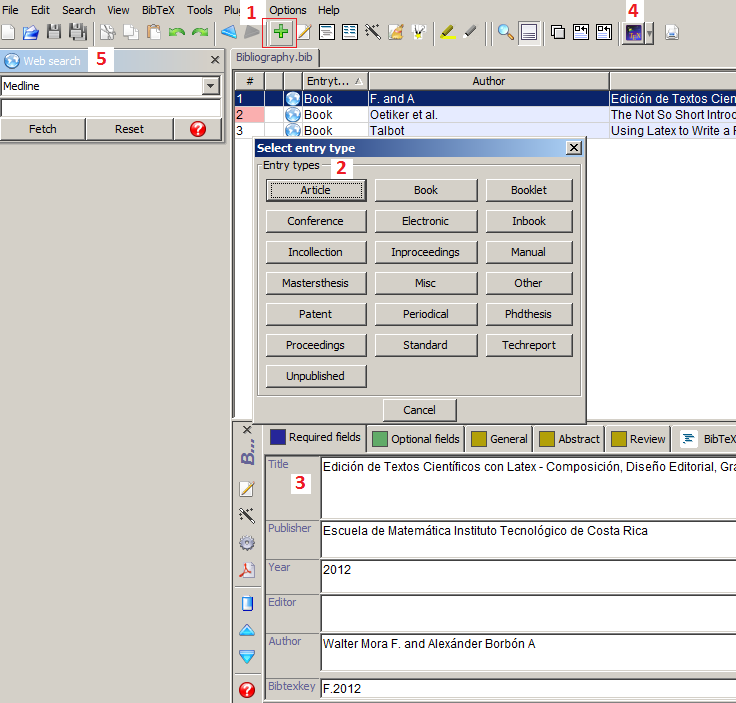
\includegraphics[width=0.7\linewidth]{Figures/Jabref1}
	\caption{Pasos de creación bibliográfica con Jabref}
	\label{fig:Jabref1}
\end{figure}

Para mas comandos revisar \href{http://en.wikibooks.org/wiki/LaTeX/Bibliography_Management#Natbib}{acá}.
\Activate
\begin{easylist}[itemize]	
	& \verb|\cite{ }|: \cite{F.2012}
	& \verb|\citep{ }|: \citep[ver][Cap. 9]{F.2012}
	& \verb|\citet{ }|: \citet{F.2012}
	& \verb|\citeauthor{ }|: \citeauthor{F.2012}
\end{easylist}
\Deactivate

\subsection{Paquetes \textit{color} y \textit{xcolor}}
Para poder usar todos los colores de ambos paquetes correctamente en todos los formatos, se empleó una condicional \verb|if/else| porque el paquete \verb|xcolor| tiene problemas con el formato \verb|Journal|, así que cuando compilas \verb|Journal| solo usará los colores del paquete \verb|color| y para el resto de los formatos usará \verb|color| y \verb|xcolor|. Más sobre los paquetes de colores \href{http://en.wikibooks.org/wiki/LaTeX/Colors}{acá}.
\lstinputlisting[language=tex, 
caption={Configuración de paquetes Color (realimentado)}, 
label={cod:configColor},
linerange={20-26}]{../Preamble/UMSAetn.cls}

Un uso simple es, \verb|{\color{red}Texto en rojo}| {\textrightarrow} {\color{red}Texto en rojo}.

\subsection{Configuración de Indice de palabras, Hyperlinks y Glosario/Acrónimos}
Debes respetar el orden que tiene; es decir, la configuración de \verb|hyperref| \textbf{después de} Indice de palabras y \textbf{antes de} Glosario/Acrónimos, de lo contrario se perderán varios \textit{hyperlinks}.
\lstinputlisting[language=tex, 
caption={Configuración Idx-Hyperref-Glo-Acr (realimentado)}, 
label={cod:configIdxGloAcr},
linerange={28-44}]{../Preamble/UMSAetn.cls}

La sección \ref{sec:GloAcr} indica como crear y usar Glosario y Acrónimos.

\subsubsection{Indizar palabras y agregar notas al pie}
El procedimiento para ambos en sencillo y va justo después de la palabra o nota que se desea agregar.

\Activate
\begin{easylist}[itemize]	
	& Indizar: \verb|palabra\index{palabra}|, \index{palabra} aparecerá en el \textit{Índice de palabras}.
	& Nota al pie:  \verb|nota1\footnote{descripción de la nota1}| = nota1\footnote{descripción de la nota1}.	
\end{easylist}
\Deactivate

\subsection{Paquete \textit{algorithm2e}}
Hay 3 tipos de \href{http://en.wikibooks.org/wiki/LaTeX/Algorithms}{paquetes pseudo-código}; \verb|algorithmic|, \verb|algorithm2e| y \verb|algorithmicx|, se escogió el 2do por ser visualmente más atractivo.

El código \ref{cod:algorithms2e} configura las opciones básicas y ademas define \verb|keywords| nuevos, para mas opciones revisar Cap. 11 de la documentación \href{http://ctan.mirrors.hoobly.com/macros/latex/contrib/algorithm2e/doc/algorithm2e.pdf}{oficial}.

\lstinputlisting[language=tex,  
caption={Paquete algorithms2e (realimentado)}, 
label={cod:algorithms2e},
linerange={46-52}]{../Preamble/UMSAetn.cls}

Código ejemplo:
\begin{lstlisting}[language=tex, caption={}, label={}]
	\begin{algorithm}[H]
	\caption{Como escribir Algoritmos}\label{alg:Algoritmo1}
	\KwData{texto}
	\KwResult{Algoritmos en \LaTeX2e }
	iniciar\;
	\While{condición 1}{
		tarea 1\;
		\eIf(\tcc*[f]{comentario}){condición 2}{
			tarea 2\;
			tarea 3\;
		}{
		tarea 4\;
		}
	}
	\end{algorithm}
\end{lstlisting}

\begin{algorithm}[H]
	\caption{Como escribir Algoritmos}\label{alg:Algoritmo1}
	\KwData{texto}
	\KwResult{Algoritmos en \LaTeX2e }
	iniciar\;
	\While{condición 1}{
		tarea 1\;
		\eIf(\tcc*[f]{comentario}){condición 2}{
			tarea 2\;
			tarea 3\;
		}{
		tarea 4\;
		}
	}
\end{algorithm}


También se puede definir \textit{Keywords} propios con \verb|\SetKwProg{Prog}{Title}{is}{end}| en el Preámbulo, código \ref{cod:algorithms2e}
\begin{lstlisting}[language=tex, caption={}, label={}]
	\begin{algorithm}[H]
	\caption{Keywords propios}\label{alg:Algoritmo2}	
	\KwIn{in}
	\KwOut{out}
	
	\Config{Libreria}{
	opciones\;
	}
	\Def{Variables}{
	var1, var2\;			
	}
	\Fn{Func1}{
	código\;
	}
	\Fn{Func2}{
	código\;
	}	
	\Main{}{
	\textbf{call} Func1\;
	\textbf{call} Func2\;	
	}
	\end{algorithm}
\end{lstlisting}


\begin{algorithm}[H]
	\caption{Keywords propios}\label{alg:Algoritmo2}	
	\KwIn{in}
	\KwOut{out}
	
	\Config{Libreria}{
		opciones\;
	}
	\Def{Variables}{
		var1, var2\;			
	}
	\Fn{Func1}{
		código\;
	}
	\Fn{Func2}{
		código\;
	}	
	\Main{}{
		\textbf{call} Func1\;
		\textbf{call} Func2\;	
	}
\end{algorithm}

Multicolumna:
\begin{lstlisting}[language=tex, caption={}, label={}]
	\begin{algorithm}[H]
	\caption{Multicolumna}\label{alg:}	
	\KwIn{in}
	\KwOut{out}
	\begin{multicols}{2}
	\Config{Libreria}{
	opciones\;
	}
	\Def{Variables}{
	var1, var2\;			
	}
	\Fn{Func1}{
	código\;
	}
	\Fn{Func2}{
	código\;
	}	
	\Main{}{
	\textbf{call} Func1\;
	\textbf{call} Func2\;	
	}
	\end{multicols}	
	\end{algorithm}
\end{lstlisting}

\begin{algorithm}[H]
	\caption{Multicolumna}\label{alg:}	
	\KwIn{in}
	\KwOut{out}
	\begin{multicols}{2}
		\Config{Libreria}{
			opciones\;
		}
		\Def{Variables}{
			var1, var2\;			
		}
		\Fn{Func1}{
			código\;
		}
		\Fn{Func2}{
			código\;
		}	
		\Main{}{
			\textbf{call} Func1\;
			\textbf{call} Func2\;	
		}
	\end{multicols}	
\end{algorithm}

\subsection{Usar otros \textit{Fonts} y usar símbolo [\degree] en \textit{mathmode}}

\lstinputlisting[language=tex, 
caption={Otros \textmyfont{fonts} y símbolo (realimentado)}, 
label={cod:font},
linerange={54-57}]{../Preamble/UMSAetn.cls}

\paragraph{Fonts:}
Se puede aplicar tres comandos, \href{http://tex.stackexchange.com/questions/25249/how-do-i-use-a-particular-font-for-a-small-section-of-text-in-my-document/25251#25251}{ref. 1} y \href{https://www.sharelatex.com/learn/Font_typefaces}{ref. 2} :
\Activate
\begin{easylist}[itemize]	
	& \verb|\verb|: no respeta los márgenes de la página pero se puede mostrar texto \textmyfont{raw} para comandos \LaTeX, e.g \verb|\comandoLatex{}|.
	& \verb|\textsf|: formato \textsf{Sans Serif} que respeta los márgenes.
	& Crear un nuevo comando con otro \textmyfont{font}, código \ref{cod:font}.	
\end{easylist}
\Deactivate

\textsf{Texto: This text is a sample text to test font families and font typefaces. This text is a sample text to test font families and font typefaces.This text is a sample text to test font families and font typefaces.}

\textmyfont{Texto: This text is a sample text to test font families and font typefaces. This text is a sample text to test font families and font typefaces.This text is a sample text to test font families and font typefaces.}

\paragraph{Símbolo [\degree]:}
En \verb|mathmode| no se puede mostrar el símbolo [\degree] con \verb|\textdegree|, entonces se recurre al paquete \verb|gensymb|.

\Activate
\begin{easylist}[itemize]	
	& \verb|\textdegree|: $temperatura = 100 [\textdegree C]$
	& \verb|\degree|: $temperatura = 100 [\degree C]$	
\end{easylist}
\Deactivate


\subsection{Paquetes gráficos: \textit{eps, Tikz/PGF y circuitikz}}
La configuración siguiente sirve para la correcta visualización de los formatos de graficación \textit{EncapsulatedPostScript} \textmyfont{(.eps)} y \textmyfont{Tikz(nativo)} para este \textmyfont{template}. En la sección \ref{sec:crear_graficos} se muestra ejemplos de aplicación.

\lstinputlisting[language=tex, 
caption={Configuración de paquetes gráficos (realimentado)}, 
label={cod:},
linerange={59-62}]{../Preamble/UMSAetn.cls}

\subsubsection{Tikz/PGF}
Aunque existe \textmyfont{PostScript(.ps)}, el más usado es \textmyfont{\href{http://www.texample.net/tikz/}{Tikz/PGF}} por la gran documentación y mejor compatibilidad con \textmyfont{pdflatex}.

En el ejemplo siguiente se muestra una señal senoidal con eje de coordenadas desde $x[-1,5],y[-1,5]$.

\begin{lstlisting}[language=tex, caption={}, label={}]
\begin{center}
\begin{tikzpicture}[scale=0.8]\shorthandoff{>}
\draw[->] (-1,0) -- (5,0) node[right] {$x$}; 
\draw[->] (0,-1) -- (0,5) node[left] {$y$};
% Dominio = a:b
\draw[smooth, domain = -1:5, color=blue]
%\x r indica que x se mide en radianes
plot (\x,{sin(\x r)}) node[right] {$y = \sin(x)$};
\draw[smooth, domain = -1:1, color=black]
plot (\x,{1.5*exp(\x)}) node[right] {$y = e^x$};
\end{tikzpicture}
\end{center}
\end{lstlisting}

\begin{center}
	\begin{tikzpicture}[scale=0.8]\shorthandoff{>}
	\draw[->] (-1,0) -- (5,0) node[right] {$x$}; 
	\draw[->] (0,-1) -- (0,5) node[left] {$y$};
	% Dominio = a:b
	\draw[smooth, domain = -1:5, color=blue]
	%\x r indica que x se mide en radianes
	plot (\x,{sin(\x r)}) node[right] {$y = \sin(x)$};
	\draw[smooth, domain = -1:1, color=black]
	plot (\x,{1.5*exp(\x)}) node[right] {$y = e^x$};
	\end{tikzpicture}
\end{center}

\subsubsection{Circuitikz}
Para mostrar esquemas y/o diseños electrónicos y eléctricos generalmente se recurre a un \textit{Software} dedicado como \textmyfont{Proteus o CircuitMaker}, pero algunos prefieren programar los esquemas desde {\LaTeX} a través de \textmyfont{circuitikz}.

\begin{lstlisting}[language=tex, caption={Ejemplo circuitikz}, label={}]
\begin{center}
\begin{circuitikz}[american]\shorthandoff{>}
\draw (0,0) 
node[ground]{}
(1.2,4.5) node[op amp] {}
(0,2) to[R,  l^=$R_4$, v_>=$V_1^+$, -*] (0,0)
(0,2)--(0,4) 
(2.5,2) to[R, l^=$R_3$, i=$i_1$] (0,2)
(2.5,2) to[short, *-](2.5,3.5)
(2.5,3.5) to[R, l^=$R_2$, -*] (4.7,3.5)
(4.7,3.5) to[R, l^=$R_1$] (6.7,3.5)
(6.7,4.5) to[short, -*, i=$i _o$] (6.7,3.5)
(2.2,4.5) to[short, -o] (7.5,4.5)
(3.5,2) node[op amp,xscale=-1] {}
(4.7,1.5) node[ground]{}
(4.7,2.5) --(4.7,3.5)
(0,5) node[ocirc] {}
{[ anchor=east] (0,5) node {$V_i$}}
{[ anchor=west] (7.5,4.5) node {$V_o$}}
{[ anchor=north] (2.5,2) node {$V_o^\prime$}};		
\end{circuitikz}
\end{center}
\end{lstlisting}

\begin{center}
	\begin{circuitikz}[american]\shorthandoff{>}
		\draw 
		(0,0) node[ground]{}
		(1.2,4.5) node[op amp] {}
		(0,2) to[R, l^=$R_4$, v_>=$V_1^+$, -*] (0,0)
		(0,2)--(0,4) 
		(2.5,2) to[R, l^=$R_3$, i=$i_1$] (0,2)
		(2.5,2) to[short, *-](2.5,3.5)
		(2.5,3.5) to[R, l^=$R_2$, -*] (4.7,3.5)
		(4.7,3.5) to[R, l^=$R_1$] (6.7,3.5)
		(6.7,4.5) to[short, -*, i=$i _o$] (6.7,3.5)
		(2.2,4.5) to[short, -o] (7.5,4.5)
		(3.5,2) node[op amp,xscale=-1] {}
		(4.7,1.5) node[ground]{}
		(4.7,2.5) --(4.7,3.5)
		(0,5) node[ocirc] {}
		{[ anchor=east] (0,5) node {$V_i$}}
		{[ anchor=west] (7.5,4.5) node {$V_o$}}
		{[ anchor=north] (2.5,2) node {$V_o^\prime$}};		
	\end{circuitikz}
\end{center}	

\begin{center}
	\begin{circuitikz}[american voltages]\shorthandoff{>}
		\draw
		(0,0) to [short, *-] (6,0)
		to [V, l_=$\mathrm{j}{\omega}_m \underline{\psi}^s_R$] (6,2) 
		to [R, l_=$R_R$] (6,4) 
		to [short, i_=$\underline{i}^s_R$] (5,4) 
		(0,0) to [open, v^>=$\underline{u}^s_s$] (0,4) 
		to [short, *- ,i=$\underline{i}^s_s$] (1,4) 
		to [R, l=$R_s$] (3,4)
		to [L, l=$L_{\sigma}$] (5,4) 
		to [short, i_=$\underline{i}^s_M$] (5,3) 
		to [L, l_=$L_M$] (5,0); 
	\end{circuitikz}
\end{center}


\begin{quote}
	Nota: Es importante agregar \verb|\shorthandoff{>}| en el código, porque por defecto \textmyfont{tikz y circuitikz} tienen problemas con \textmyfont{babel spanish}, ref. \href{http://tex.stackexchange.com/questions/105930/how-to-put-label-and-voltage-on-same-object-in-circuitikz/105996#105996}{error circuitikz},
	\href{http://www.texample.net/tikz/examples/tag/circuitikz/}{ejemplos}, \href{ctan.mackichan.com/graphics/pgf/contrib/circuitikz/circuitikzmanual.pdf}{manual} e \href{https://www.sharelatex.com/learn/CircuiTikz_package}{info}. 
\end{quote}

Como siempre, se recomienda leer la \href{http://www.texample.net/media/pgf/builds/pgfmanualCVS2012-11-04.pdf}{documentación oficial}, \href{http://en.wikibooks.org/wiki/LaTeX/PGF/TikZ}{introducción} y revisar \href{http://www.texample.net/tikz/examples/}{ejemplos} de interés.

\subsubsection{Herramientas externas}
Hay un gran numero de \textit{Software} dedicado para graficar en {\LaTeX}, \href{https://wiki.gnome.org/Apps/Dia}{Dia} para varios formatos, \href{http://www.tikzedt.org/}{TikzEdt} para \textmyfont{Tikz/PGF},  \href{http://latexdraw.sourceforge.net/}{LatexDraw} para \textmyfont{.ps}, la elección depende de la finalidad y gustos. Ref. \href{http://tex.stackexchange.com/questions/26972/what-gui-applications-are-there-to-assist-in-generating-graphics-for-tex}{Lista 1} y \href{http://tex.stackexchange.com/questions/205/what-graphics-packages-are-there-for-creating-graphics-in-latex-documents}{Lista 2}

\begin{figure}[H]
	\centering
	\subfigure[Dia]{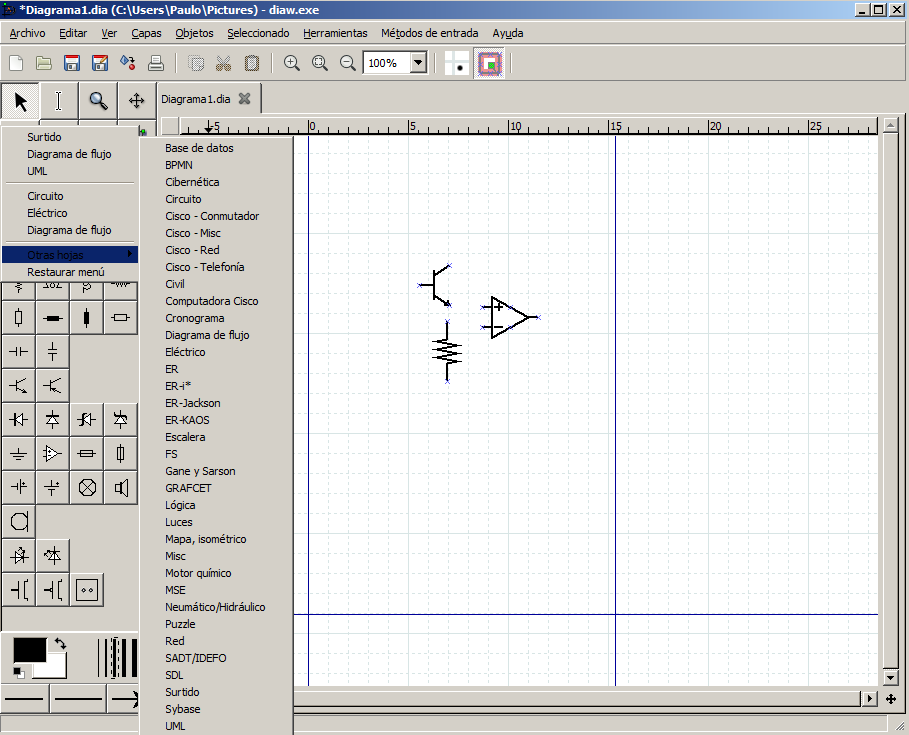
\includegraphics[width=0.7\linewidth]{Figures/Dia}}
	\subfigure[TikzEdt]{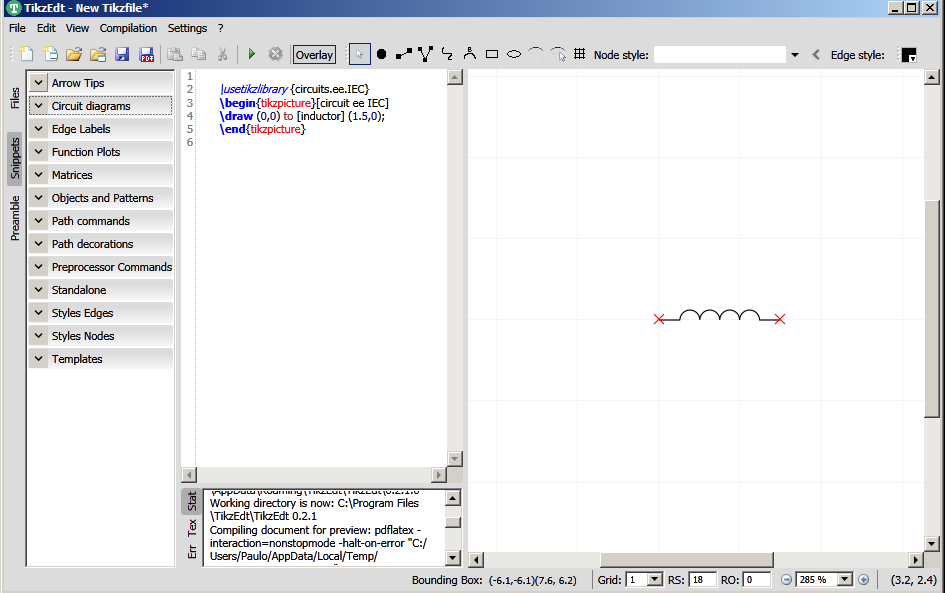
\includegraphics[width=0.7\linewidth]{Figures/TikzEdt}}
	\subfigure[LatexDraw]{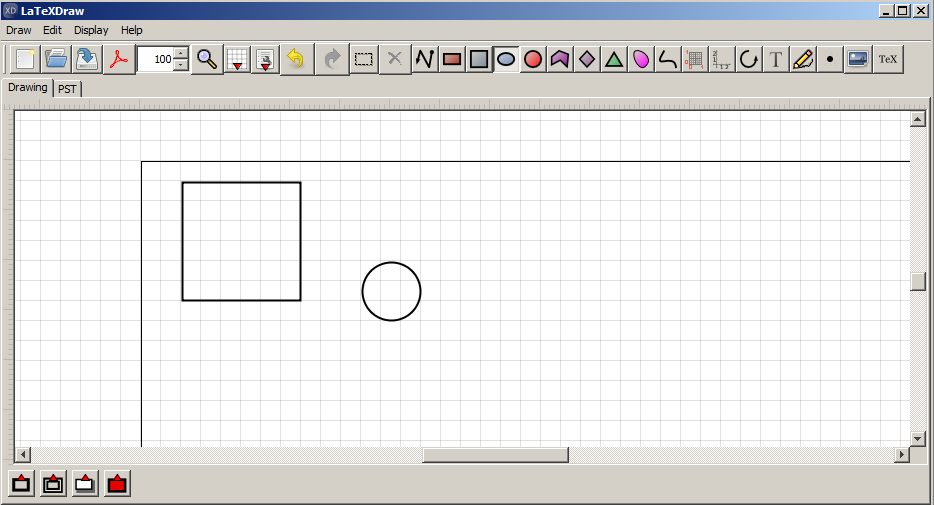
\includegraphics[width=0.7\linewidth]{Figures/LatexDraw}}
	\caption{Herramientas externas}
	\label{}
\end{figure}


\subsection{Animaciones con GNUplot}
\href{http://www.gnuplot.info/}{GNUplot} es un entorno de graficación por lineas de comando, multiplataforma y usado por \textmyfont{Octave}.

\lstinputlisting[language=tex, 
caption={Configuración de Animaciones con GNUplot(realimentado)}, 
label={cod:},
linerange={64-82}]{../Preamble/UMSAetn.cls}

Para trabajar con {\LaTeX}:
\Activate
\begin{easylist}[itemize]	
	& \href{http://www.gnuplot.info/download.html}{Descargar} \textmyfont{GNUplot}
	& Configurar la instalación según la fig. \ref{fig:gnuplot}(a).
	& Agregar en entornos de variable de \textmyfont{Windows} \verb|C:\Program Files\gnuplot\bin|, fig. \ref{fig:gnuplot}(b)
	& Compilar con \textmyfont{arara}.
	& Abrir \textmyfont{Thesis.pdf} con \textmyfont{Adobe 6} o superior. No se podrá visualizar en \textmyfont{Foxit Reader} o \textmyfont{Phantom Reader}.	 	
\end{easylist}
\Deactivate

\begin{figure}[H]
	\centering
	\subfigure{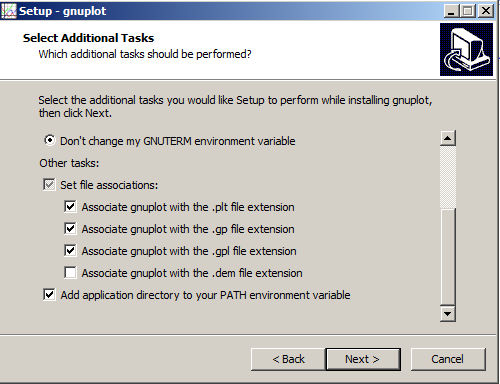
\includegraphics[width=0.48\linewidth]{Figures/gnuplot1}}
	\subfigure{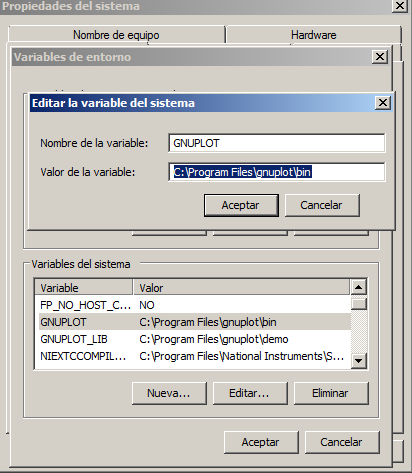
\includegraphics[width=0.48\linewidth]{Figures/gnuplot2}}
	\caption{Configuración GNUplot}
	\label{fig:gnuplot}
\end{figure}



\newcommand{\mainaxis}{
	% Main axis
	\draw (-2, 0) -- (2, 0) (0, 0) -- (0, 1.15);
	
	% Small tickmarks on the x axis
	\foreach \x in {-2,-1.9,...,2} {
		\draw (\x, 0) -- (\x, -0.8pt);
	}
	
	% Labels on the $x$ axis; the llap makes the label center on the
	% number without the minus.
	\foreach \x/\label in {-2/\llap{$-$}2,-1/\llap{$-$}1,0/0,1/1,2/2} {
		\node[x tick label] at (\x, 0) {$\label$};
		\draw[major tick] (\x, 0) -- (\x, -1.25pt);
	}
	
	% Y tick mark.
	\draw[major tick] (-1.25pt,.5) -- (0,.5);
	
	% Y labels.
	\node[y tick label] at (0,.5) {$\frac{1}{2}$};
	\node[y tick label] at (0,1) {$1$};
}

\def\yshift{-2cm} % Shift of the lower axis
\newcommand{\drawaxes}{
	\mainaxis
	\node[axis label] at (2,0) {$\scriptstyle \tau$};
	
	% Second axis, where the convultion will be drawn.
	\begin{scope}[yshift=\yshift]
		\foreach \y in {0.1,0.2,...,1.0}
		\draw[black!20] (-2,\y) -- (2,\y);
		\mainaxis
		\node[axis label] at (2,0) {$\scriptstyle t$};
	\end{scope}
	
	\begin{pgfonlayer}{foreground}
		\node at (0,1.25) {$f$};
		\node[anchor=base] at (0,-.55)
		{$f*g =\!\!\displaystyle\int\limits_{-\infty}^{\infty}
			\!\!f(\tau)g(t-\tau)\,d\tau$};
	\end{pgfonlayer}
	
	\draw[major tick] (-1.25pt,.5) -- (0,.5) (-1.25pt,1) -- (0,1);
	
	% f(\tau) is basically fixed.
	\draw[function f] (-0.5, 0) -- +(0,1) -- +(1,1) -- +(1,0);
	\clip (-2,-2) rectangle (2, 1.75);
}

\newcommand{\drawg}[1]{
	\draw[function g] (#1,0) ++(-0.5, 0) -- +(0,1) -- +(1,1) -- +(1,0);
	\draw[function g position] (#1,1.4) -- (#1,\yshift);
	\node[fill=white] at (#1, 1.25) {$g$};
	
	% We now slightly abuse \ifdim to determine whether
	% there's an overlap.
	\ifdim#1pt>-1pt\ifdim#1pt<1.01pt
	% Draw legend.
	\fill[overlap] (-2,1.51) rectangle +(0.15,0.15);
	% The right side of f overlaps with the left side of g:
	% 'entering'
	\ifdim#1pt<0pt
	\node[anchor=west] at (-1.85, 1.575)
	{$f(\tau)g(\pgfmathprintnumber{#1} - \tau$)};
	\begin{pgfonlayer}{background}
		\fill[overlap] (-.5,0) rectangle (#1+.5,1);
	\end{pgfonlayer}
	\draw[convolution] (-1,\yshift) -- (#1, \yshift+1cm+#1 cm);
	\else
	% The left side of f overlaps with the right side of g:
	% 'leaving'
	\node[anchor=west] at (-1.85, 1.575)
	{$f(\tau)g(\pgfmathprintnumber{#1} - \tau$)};
	\begin{pgfonlayer}{background}
		\fill[overlap] (#1-.5,0) rectangle (.5,1);
	\end{pgfonlayer}
	\draw[convolution] (-1,\yshift) -- +(1, 1) --
	(#1,\yshift+1cm-#1 cm);
	\fi
	\else
	% 'g' is completely past 'f', draw the result.
	\draw[convolution] (-1,\yshift) -- +(1,1) -- +(2,0);
	\fi\fi
}

\begin{figure}[H]
	\begin{center}	
		\begin{animateinline}[controls,
			autoplay,buttonsize=1.2em,
			buttonbg=0.6:0.6:1,buttonfg=0.2:0.2:1,
			begin={\begin{tikzpicture}[scale=2]\drawaxes},
			end={\end{tikzpicture}}]{8}
			
			% Generate frames for -2 ... 2
			\xdef\pos{-2}
			\whiledo{\lengthtest{\pos pt < 2.1 pt}}{
				\drawg{\pos}\newframe
				\pgfmathsetmacro{\pos}{\pos + 0.1}
				\xdef\pos{\pos}
			}
			
			\drawg{\pos}
		\end{animateinline}
	\end{center}
	\caption{Ejemplo de animación con GNUplot}
	\label{fig:}        
\end{figure}

\subsection{Paquete \textit{Codehighlighting} (colorear códigos)}
Son 3 paquetes que se probó, \verb|Listing|, \verb|verbment| y \verb|minted|, el primero es nativo pero \verb|verbment| y \verb|minted| requieren \verb|Python/Pygments|. 	

\subsubsection{Paquete \textit{listings}}
\verb|Verbments| fue el primer paquete que compiló, luego intenté con \verb|minted| sin resultados satisfactorios, al final le dí una oportunidad a \verb|listings| y funcionó sin problemas, si deseas puedes revisar los siguientes links, \href{http://tex.stackexchange.com/questions/102596/minted-vs-texments-vs-verbments}{minted-vs-texments-vs-verbments}, \href{http://tex.stackexchange.com/questions/23458/how-to-install-syntax-highlight-package-minted-on-windows-7}{minted-on-windows-7}, la documentación \href{http://www.ctan.org/pkg/verbments}{oficial} y \cite[ver][Cap. 9.8]{F.2012}. 

\verb|Listings| demostró ser el mas cómodo para colorear códigos, recomiendo leer la documentación \href{http://www.ctan.org/tex-archive/macros/latex/contrib/listings/}{oficial} y revisar este \href{http://en.wikibooks.org/wiki/LaTeX/Source_Code_Listings}{link.}

La configuración \ref{cod:configlistings} del paquete puede ser larga pero permite crear un estilo propio.  
\lstinputlisting[language=tex, 
caption={Configuración listings (realimentado)}, 
label={cod:configlistings},
linerange={84-139}]{../Preamble/UMSAetn.cls}

Para mostrar código directamente una configuración simple sería:
\begin{verbatim}
\usepackage{listings}[language=c, caption={}, label={}]
\begin{lstlisting}
#include <stdio.h>
#define N 10
/* Block
* comment */

int main()
{
int i;

// Line comment.
puts("Hello world!");

for (i = 0; i < N; i++)
{
puts("LaTeX is also great for programmers!");
}

return 0;
}
\end{lstlisting}
\end{verbatim}

cuyo resultado es:
\begin{lstlisting}[language=c, caption={}, label={}]
#include <stdio.h>
#define N 10
/* Block
* comment */

int main()
{
int i;

// Line comment.
puts("Hello world!");

for (i = 0; i < N; i++)
{
puts("LaTeX is also great for programmers!");
}

return 0;
}
\end{lstlisting}

También se puede imprimir el código contenido en un documento, lo que es muy útil cuando existen constantes cambios en tu proyecto (este es el método que se aplica en este \verb|Template|, revisar \ref{quo:Importante})
\begin{lstlisting}[language=tex, caption={}, label={}]
\lstinputlisting[language=c, caption={test.c}, label={test.c}]{Codes/test.c}
\end{lstlisting}

pero si se usa un \href{http://en.wikibooks.org/wiki/LaTeX/Source_Code_Listings#Automating_file_inclusion}{macro automatizado}, entonces se simplifica aun más, ref. \href{ http://en.wikibooks.org/wiki/LaTeX/Macros#New_commands}{macros{\LaTeX}}. 
\lstinputlisting[language=tex, 
caption={Macro listings (realimentado)}, 
label={cod:macrolistings},
linerange={140-142}]{../Preamble/UMSAetn.cls}

invocando el nuevo comando.
\begin{lstlisting}[language=tex, caption={}, label={}]
\includecode{c}{Codes/test.c}% c=language, Codes/test.c=ubicación del documento
\end{lstlisting}

se obtiene el código \ref{Codes/test.c}.
\includecode{c}{Codes/test.c}

\label{rangocodigo}para imprimir en un rango de lineas se usa \verb|linerange|, por ejemplo si deseo imprimir de la linea 1 a la 7 de \verb|Codes/test.c|, entonces aplico 
\begin{lstlisting}[language=tex, caption={}, label={}]
\lstinputlisting[language=c, 
	caption={test.c}, 
	label={test.c}, 
	linerange={1-7}]{Codes/test.c}
\end{lstlisting}

y quedaría como el código \ref{cod:Rangotest.c}. 
\lstinputlisting[language=c, 
caption={Rango test.c}, 
label={cod:Rangotest.c},
linerange={1-7}]{Codes/test.c}

\subsection{Paquete \textit{kvoptions}}
Esta es la parte central del código, el uso del paquete \verb|kvoptions| permite crear clases \verb|.cls| y estilos \verb|.sty| de una forma cómoda, haciendo uso de prefijos y comandos para crear opciones al momento de usar la clase \verb|UMSAetn.cls| 

Primero se crea las opciones \verb|Keyval| por familia y prefijo para usar como \verb|prefix@option|, luego se lista todas las opciones como:
\Activate
\begin{easylist}[itemize]	
	& \verb|DeclareBoolOption|: es una condicional falso o verdadero para escoger la opción correspondiente, e.g. \verb|\documentclass[Journal]| compilará un documento tipo \verb|Journal|.
	& \verb|DeclareStringOption|: requiere un argumento, e.g. \verb|\documentclass[Journal, FontSize=10pt|, tamaño del \textit{font} 10pt
\end{easylist}
\Deactivate 

\lstinputlisting[language=tex, 
caption={Configuración \textit{kvoptions} (realimentado)}, 
label={cod:configKvoptions},
linerange={145-158}]{../Preamble/UMSAetn.cls}

\subsubsection{Opción \textit{Journal}}
Se carga como clase tipo \verb|report| con la inclusión del paquete \verb|pax| y \verb|pdfpages| necesarios para compilar varios artículos sin perder sus \textit{hyperlinks} correspondientes.

\lstinputlisting[language=tex, 
caption={Configuración opción Journal (realimentado)}, 
label={cod:configkvoptions},
linerange={160-188}]{../Preamble/UMSAetn.cls}

\paragraph{Paquete \textit{Fancy header}:}
Permite personalizar la cabecera y pie de página para todo el documento, es versátil pero requiere una lectura de las opciones y estilos que maneja, puedes consultar en \cite{Oetiker2014} y \href{http://www.sharelatex.com/learn/Management_in_a_large_project}{ref. 1}, \href{http://en.wikibooks.org/wiki/LaTeX/Page_Layout#Customizing_with_fancyhdr}{ref. 2}.

\paragraph{Makechapterhead:}
Redefine las clases \verb|book| y \verb|report| sin alterar el TOC para eliminar la palabra \verb|Capítulo|, \href{http://tex.stackexchange.com/questions/62516/how-to-suppress-chapter-in-chapter-while-keeping-numbering/62527#62527}{ref.}

Capítulo 1. Introducción\\
Capítulo 2. Antecedentes\\
Capítulo 3. Conclusiones\\
por\\
1. Introducción\\
2. Antecedentes\\
3. Conclusiones\\

Al compilar \verb|Journal o Thesis| se puede ver su efecto.

\subsubsection{Opción \textit{Article}}
Se cargar como clase tipo \verb|article| con dos columnas, con el paquete \verb|titlesec| se redefine el tipo de letra y numeración para los títulos y subtítulos.

\verb|PageType| es el comando para numerar o no enumerar las páginas del Articulo, los argumentos son \verb|empty| para \verb|Journal| y \verb|plain| para \verb|Article Standalone|.

\lstinputlisting[language=tex, 
caption={Configuración opción Article (realimentado)}, 
label={cod:configkvoptions},
linerange={190-207}]{../Preamble/UMSAetn.cls}

\subsubsection{Opción \textit{Profile}}
Se carga como clase tipo \verb|Article| de una sola columna, el uso del paquete \verb|parskip| agrega una fila vacía después de cada párrafo y \verb|setlenght| define el \textit{indent = 0 (default 15pt)}, \href{http://en.wikibooks.org/wiki/LaTeX/Paragraph_Formatting}{ref.}

\lstinputlisting[language=tex, 
caption={Configuración opción Profile (realimentado)}, 
label={cod:configkvoptions},
linerange={209-216}]{../Preamble/UMSAetn.cls}

\subsubsection{Opción \textit{Thesis}}
Utiliza la clase \verb|book| y salto de línea e \textit{indent = 0}. 

\lstinputlisting[language=tex, 
caption={Configuración opción Thesis (realimentado)}, 
label={cod:configkvoptions},
linerange={218-261}]{../Preamble/UMSAetn.cls}

\subsubsection{Opción \textit{Tutorial}}
Utiliza la clase \verb|article| y salto de línea e \textit{indent = 0}. 

\lstinputlisting[language=tex, 
caption={Configuración opción Tutorial (realimentado)}, 
label={cod:configkvoptions},
linerange={263-270}]{../Preamble/UMSAetn.cls}

\section{Preamble/Administrative.sty}
Define los argumentos de las opciones respectivas al implementar la clase, opciones \textsf{generales, Journal, Article y Thesis/Profile/Tutorial} y con el comando \verb|\ProcessKeyvalOptions{admin}|  se procesa todos los \verb|keyvlas|.

\lstinputlisting[language=tex, 
caption={Preamble/Administrative.sty (realimentado)}, 
label={cod:Administrative},
linerange={1-49}]{../Preamble/Administrative.sty}

Después de procesar los \verb|keyvals| se define los comandos para las opciones.

\lstinputlisting[language=tex, 
caption={Preamble/Administrative.sty (realimentado)}, 
label={cod:Administrative},
linerange={51-132}]{../Preamble/Administrative.sty}

\section{Backpages/Glossary.tex y Backpages/Acronyms.tex}\label{sec:GloAcr}
Tampoco requieren explicación pero puedes consultar sobre Acrónimos/Glosarios y algunas opciones en \href{http://www.sharelatex.com/learn/Glossaries}{Glossaries} y \href{http://www.dickimaw-books.com/latex/thesis/html/makeglossaries.html}{makeglossaries}.
 
Comandos para Glosarios:
\Activate
\begin{easylist}[itemize]	
& \verb|\gls{ }| Imprime en minúsculas, \gls{latex}
& \verb|\Gls{ }| Primera letra mayúscula, \Gls{latex}
& \verb|\glspl{ }| Minúsculas en plural, \glspl{latex}
& \verb|\Glspl{ }| Primera letra mayúscula y en plural, \Glspl{latex}	
\end{easylist}
\Deactivate

Comandos para Acrónimos:
\Activate
\begin{easylist}[itemize]	
& \verb|\acrlong{ }| Imprime la descripción, \acrlong{CAD} 
& \verb|\acrshort{ }| Solo el acrónimo, \acrshort{CAD} 
& \verb|\acrfull{ }| Ambos, \acrfull{CAD}
\end{easylist}
\Deactivate

\section{Formato JournalIEA.tex}
El formato \verb|JournalIEA.tex| usa \verb|pdfpages| para incluir los artículos como \verb|pdf| y \verb|pax| para recuperar los \textit{hyperlinks} de los mismos.
\lstinputlisting[language=tex, 
caption={Formato JournalIEA.tex (realimentado)}, 
label={cod:}]{../JournalIEA/JournalIEA.tex}

\subsection{Paquete \textit{Pax}}
El objetivo de usarlo en este template es para agregar todos los \verb|artículos.pdf| sin perder los \textit{hyperlinks} y 'referencias cruzadas', los pasos para compilar correctamente son:

\Activate
\begin{easylist}[itemize]	
	& Instalar \verb|pax| desde \verb|MiKTeX Package Manager|.
	& Instalar \verb|strawberry perl| x86 o x64.
	& Descargar \verb|PDFBox-0.7.3| desde \url{http://prdownloads.sourceforge.net/pdfbox/PDFBox-0.7.3.zip?download},         \url{http://sourceforge.net/project/showfiles.php?group_id=78314}
	& Descomprimir en \verb|C:\PDFBox-0.7.3|
	& Agregar a entorno de \textbf{variables del sistema}: 
	&& \verb|C:\Program Files (x86)\MiKTeX 2.9\scripts\pax|  
	&& \verb|C:\PDFBox-0.7.3\lib|
	& Actualizar paquetes de \verb|MiKTeX| con \verb|Update (admin)|
	& Ejecutar \verb|Refresh FNDB y Update Formats|  
	& Reiniciar PC	
	& Con \verb|cmd| entrar a \verb|C:\Program Files (x86)\MiKTeX 2.9\scripts\pax| \\y ejecutar \verb|perl pdfannotextractor.pl --install|
	& Si pide \verb|wget| o \verb|curl|, descargar y copiar \verb|curl.exe| en \\\verb|C:\Program Files (x86)\MiKTeX 2.9\scripts\pax|
	& Si pide \verb|unzip|, instalar \verb|unzip-5.51-1|, copiar todos los archivos relacionados con \textsf{unzip.exe} incluyendo a \verb|unzip32.dll| de la carpeta \verb|C:\Program Files (x86)\GnuWin32\bin| \\ a \verb|C:\Program Files (x86)\MiKTeX 2.9\scripts\pax|
	& Desde \verb|cmd|:
	&& Entrar a la carpeta \verb|ArticlesIEA/Article1| con el comando \verb|cd|
	&& Ejecutar: \verb|java -cp "C:\Program Files (x86)\MiKTeX 2.9\scripts\pax\pax.jar;|\\\verb|C:\PDFBox-0.7.3\lib\PDFBox-0.7.3.jar" pax.PDFAnnotExtractor Article1.pdf| 	
	& Se creara \verb|Article1.pax|
	& Abrir \verb|JournalIEA.tex| y compilar con \verb|pdflatex| o \verb|arara|.
	& Listo, se recuperarán los \textit{hyperlinks} y se unirá todo el documento \verb|Journal|
\end{easylist}
\Deactivate

\section{Formato Article1.tex}
Se puede copiar la carpeta \verb|Article1| cuantos artículos sean necesarios para el \textsf{Journal}, \textbf{PageType} es importante porque indica si ese Artículo se usará para \textsf{Journal} o solo será un Artículo independiente, la opción \textsf{plain} enumera cada página para Artículo independiente y \textsf{empty} no enumera ninguna página para poder usarlo en un \textsf{Journal}.
\lstinputlisting[language=tex, 
caption={Formato Article1.tex (realimentado)}, 
label={cod:}]{../ArticlesIEA/Article1/Article1.tex}

\section{Formato Profile.tex}
\lstinputlisting[language=tex, 
caption={Formato Profile.tex (realimentado)}, 
label={cod:}]{../Profile/Profile.tex}

\section{Formato Thesis.tex}
\lstinputlisting[language=tex, 
caption={Formato Thesis.tex (realimentado)}, 
label={cod:}]{../Thesis/Thesis.tex}

\section{Formato MainTutorial.tex}
\lstinputlisting[language=tex, 
caption={Formato MainTutorial.tex (realimentado)}, 
label={cod:}]{../Tutorial/MainTutorial.tex}

\section{Modo matemático}
La notación básica de texto matemático es \verb|$x=2y$| $x=2y$.

Centrado:
\verb|$$ {x}^{2}+{y}^{z}={z}^{2} $$|
$$ {x}^{2}+{y}^{z}={z}^{2} $$

\subsection{TeXstudio/Wizards/MathAssistant}
\verb|TeXstudio| ofrece los comandos matemáticos en su barras laterales y ademas tiene integrado un asistente en \verb|Wizards/MathAssistant| fig. \ref{fig:TeXstudioMath}
\begin{figure}[H]
	\centering
	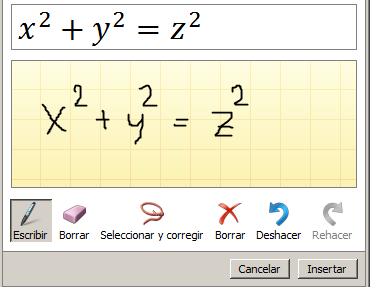
\includegraphics[width=0.3\linewidth]{Figures/TeXstudioMath}
	\caption{Asistente matemático de TeXstudio.}
	\label{fig:TeXstudioMath}
\end{figure}

Después de agregar con la tecla \verb|Insert|, muestra \verb|${x}^{2}+{y}^{2}={z}^{2}$| y resultará ${x}^{2}+{y}^{2}={z}^{2}$.

\subsection{Entorno \textit{equation}}
Ecuaciones numeradas y centradas.

\begin{lstlisting}[language=tex, caption={}, label={}]
\begin{equation}
	\log_{2}(xy)=\log_2x + \log_2y
\end{equation}

\begin{equation}
	\log_{2}(a^b)=b\log_2a
\end{equation}
\end{lstlisting}

\begin{equation}
\log_{2}(xy)=\log_2x + \log_2y
\end{equation}
\begin{equation}
\log_{2}(a^b)=b\log_2a
\end{equation}


\subsection{Entorno \textit{align}}
Alineamiento y desarrollo de ecuaciones.

\Activate
\begin{easylist}[itemize]	
	& \verb|&=| establece una igualdad en una misma columnas mientras que \verb|&| establece un cambio de columna.
	& El comando \verb|\intertext{texto}| intercala texto entre filas mientras mantiene las columnas alineadas.	
\end{easylist}
\Deactivate

\begin{lstlisting}[language=tex, caption={}, label={}]
\begin{align}
	\intertext{Agrupamos,}
	\frac{a+ay+ax+y}{x+y} & = \frac{ax+ay+x+y}{x+y}  & \mbox{Agrupar}      \nonumber \\ 
	\intertext{sacamos el factor común,}
	                      & = \frac{a(x+y)+x+y}{x+y} & \mbox{Factor común} \nonumber \\
	                      & = \frac{(x+y)(a+1)}{x+y} & \mbox{Simplificar}  \nonumber \\
	                      & = a+1                    &
\end{align}
\end{lstlisting}

\begin{align}
	\intertext{Agrupamos,}
	\frac{a+ay+ax+y}{x+y} & = \frac{ax+ay+x+y}{x+y}  & \mbox{Agrupar}      \nonumber \\ 
	\intertext{sacamos el factor común,}
	                      & = \frac{a(x+y)+x+y}{x+y} & \mbox{Factor común} \nonumber \\
	                      & = \frac{(x+y)(a+1)}{x+y} & \mbox{Simplificar}  \nonumber \\
	                      & = a+1                    &
\end{align}


\subsection{Entorno \textit{eqnarray}}
Tiene problemas con los espacios blancos, por eso se recomienda \verb|align|.

\begin{lstlisting}[language=tex, caption={}, label={}]
% Numeración selectiva
\begin{eqnarray}
y=\sqrt[n]{x} & \Longrightarrow & y^n = x \nonumber\\
			  & \Longrightarrow & n\log \,y= \log \,x, \; \mbox{si}\; x>0,\; y>0\\
			  & \Longrightarrow & \log \sqrt[n]{x}={1 \over n}\log \,x
\end{eqnarray}
\end{lstlisting}
% Numeración selectiva
\begin{eqnarray}
y=\sqrt[n]{x} & \Longrightarrow & y^n = x \nonumber\\
			  & \Longrightarrow & n\log \,y= \log \,x, \; \mbox{si}\; x>0,\; y>0\\
			  & \Longrightarrow & \log \sqrt[n]{x}={1 \over n}\log \,x
\end{eqnarray}



\section{Insertar tablas, figuras y subfiguras}
\subsection{Insertar Tablas}
Con la ayuda de \verb|TeXstudio/Wizard/QuickTabular|, \verb|QuickTabbing| y \verb|QuickArray| es bastante fácil insertar tablas, pero si requiere un poco mas de modificación como; unión de columnas y color de filas se añade algunos comandos, código \ref{cod:TablaModificada}.

\begin{lstlisting}[language=tex, caption={Insertar tabla modificada}, label={cod:TablaModificada}]
\begin{table}[H]
\centering
\begin{tabular}{c|cc}
\rowcolor{Aquamarine}  \multicolumn{3}{c}{\textbf{3 Columnas unidas}} \\ \hline
\rowcolor{LightBlue2} \textbf{Tipo} & \textbf{Modo} & \textbf{Opción} \\ \hline
A & X  & YZ \\ 
B & XZ & Y  \\ 
C & XY & Z  \\ 			 
\end{tabular} 
\caption{Ejemplo tabla modificada}
\label{tbl:insertarTbl1}
\end{table}
\end{lstlisting}

\begin{table}[H]
	\centering
	\begin{tabular}{c|cc}
		\rowcolor{Aquamarine}  \multicolumn{3}{c}{\textbf{3 Columnas unidas}} \\ \hline
		\rowcolor{LightBlue2} \textbf{Tipo} & \textbf{Modo} & \textbf{Opción} \\ \hline
		A & X  & YZ \\ 
		B & XZ & Y  \\ 
		C & XY & Z  \\ 			 
	\end{tabular} 
	\caption{Ejemplo tabla modificada}
	\label{tbl:insertarTbl1}
\end{table}

\subsection{Insertar Figuras}
Nuevamente aplicando \verb|TeXstudio/Wizard/InsertGraphics| es cómodo insertar una figura, código \ref{cod:insertarFig}.

\begin{lstlisting}[language=tex, caption={Insertar figura}, label={cod:insertarFig}]
\begin{figure}[h]
\centering
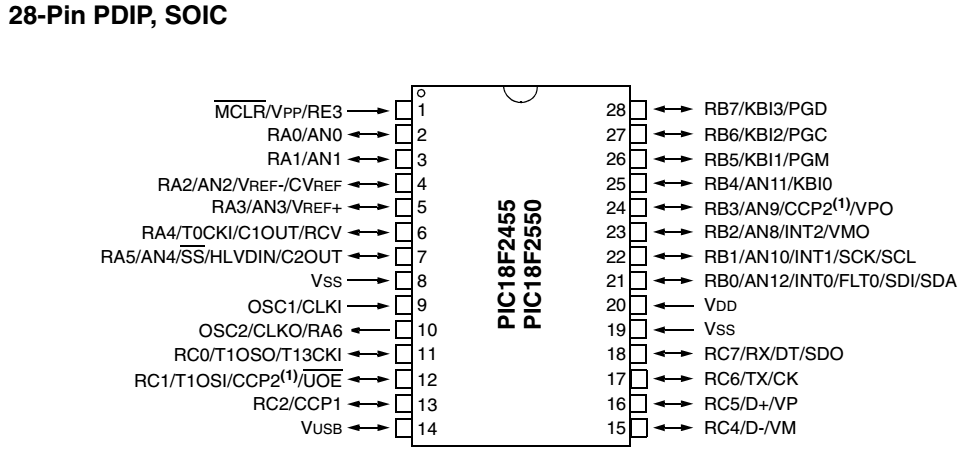
\includegraphics[width=0.45\linewidth]{Figures/18FXX5X_28PIN}
\caption{18FXX5X_28PIN}
\label{fig:18FXX5X_28PIN}
\end{figure}
\end{lstlisting}

\verb|[h]| indica la posición \verb|[here, top, bottom]|, aunque de todas formas {\LaTeX} posiciona automáticamente de acuerdo al espacio vacío y formato de la hoja.

\subsection{Paquete \textit{float}}
Sin embargo, a veces es necesario que una figura este después de un párrafo, entonces se usa \verb|\usepackage{float}| en el Preámbulo, y se cambia la opción \verb|[h]| por \verb|[H]| para poner la fig. \ref{fig:18FXX5X_28PIN} exactamente debajo de este párrafo.

\begin{figure}[H]
	\centering
	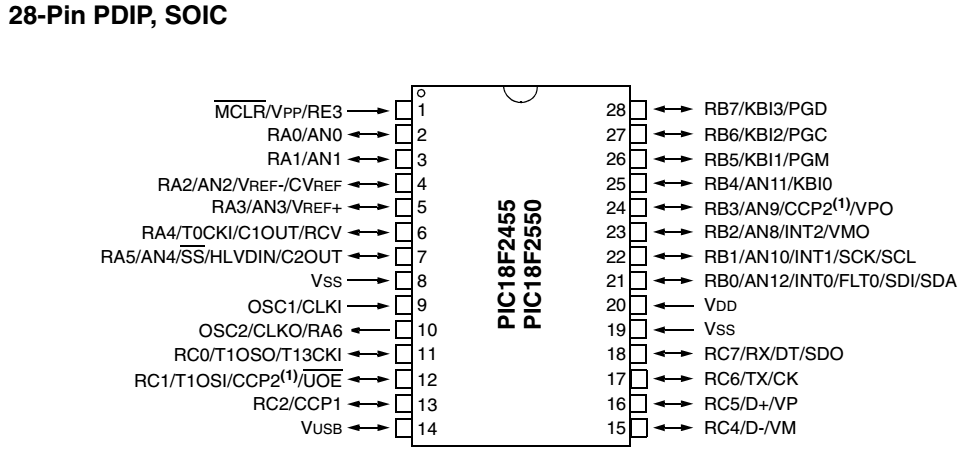
\includegraphics[width=0.45\linewidth]{Figures/18FXX5X_28PIN}
	\caption{18FXX5X 28PIN}
	\label{fig:18FXX5X_28PIN}
\end{figure}

\subsection{Subfiguras}
Las subfiguras son útiles cuando se agrupan figuras de la misma clase, se agrega \verb|\usepackage{subfigure}| en el Preámbulo y se carga de acuerdo al código \ref{cod:insertarSubfig} y quedará como la fig. \ref{fig:18FXX5X}.

\begin{lstlisting}[language=tex, caption={Insertar subfigura}, label={cod:insertarSubfig}]
\begin{figure}[H]
\centering
\subfigure[28 Pines]{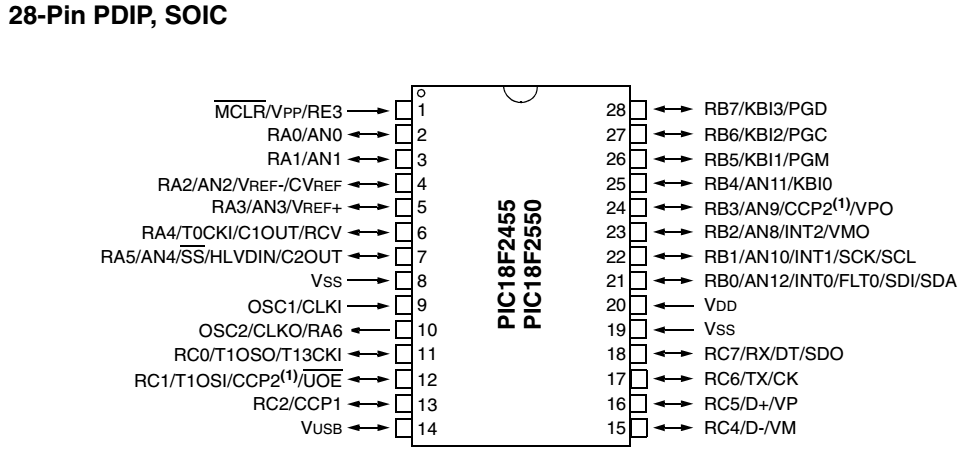
\includegraphics[width=0.45\linewidth]{Figures/18FXX5X_28PIN}}
\subfigure[40 Pines]{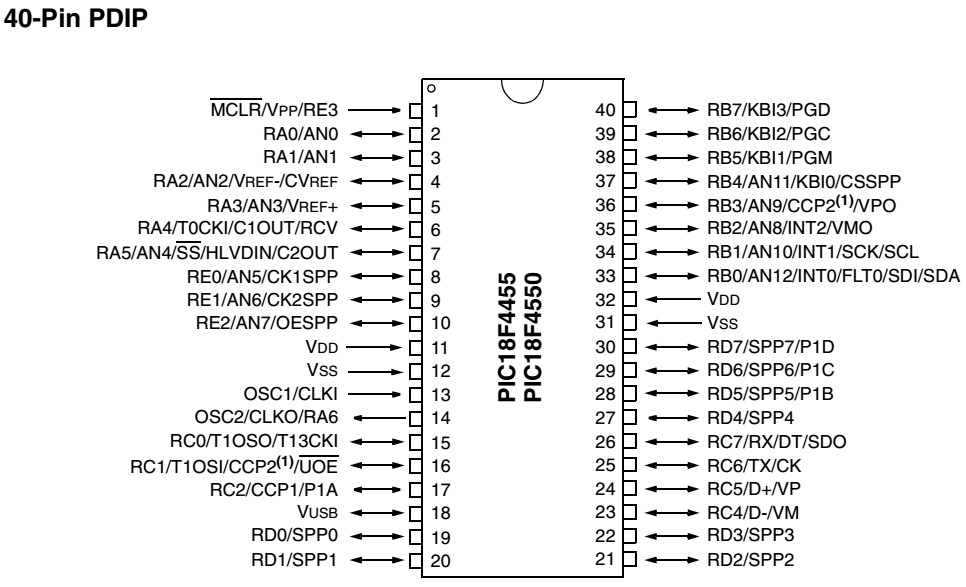
\includegraphics[width=0.45\linewidth]{Figures/18FXX5X_40PIN}}
\caption{Familia 18FXX5X}
\label{fig:18FXX5X}
\end{figure}
\end{lstlisting}

\begin{figure}[H]
	\centering
	\subfigure[28 Pines]{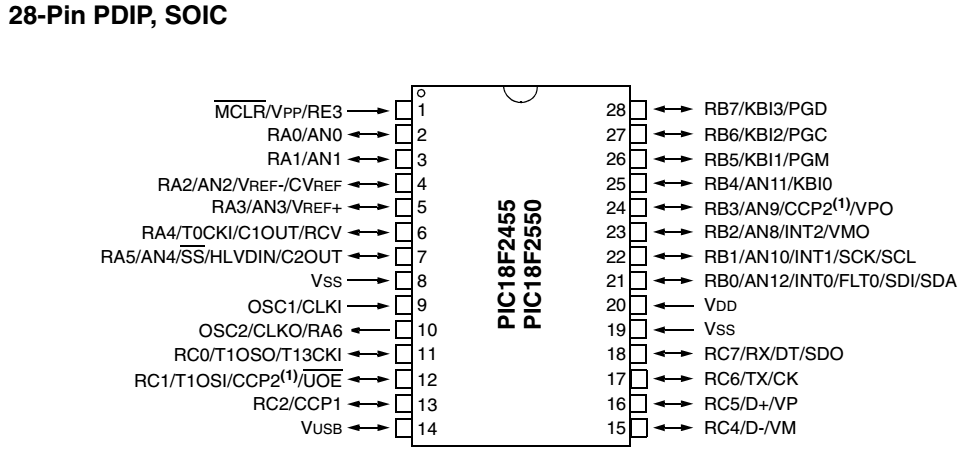
\includegraphics[width=0.45\linewidth]{Figures/18FXX5X_28PIN}}
	\subfigure[40 Pines]{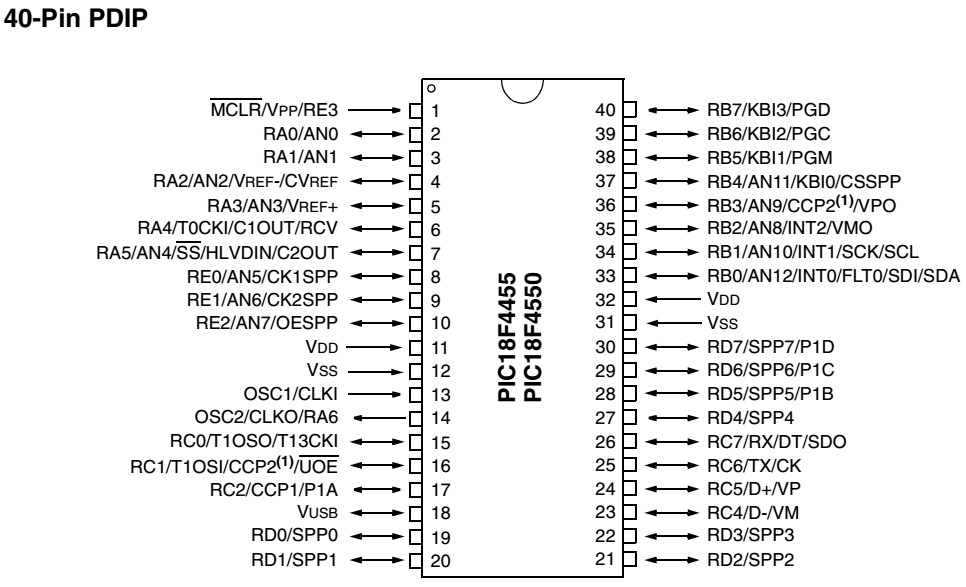
\includegraphics[width=0.45\linewidth]{Figures/18FXX5X_40PIN}}
	\caption{Familia 18FXX5X}
	\label{fig:18FXX5X}
\end{figure}

\section{Repositorios de \textit{Templates} y recomendaciones}
Antes de crear este \verb|Template| busque y probé otros en repositorios como \url{https://www.sharelatex.com/templates/} y \url{http://www.latextemplates.com/}, donde encontré 3 \verb|Templates| interesantes.
\Activate
\begin{easylist}[itemize]	
	& \href{http://www.latextemplates.com/template/masters-doctoral-thesis}{Masters/Doctoral Thesis} se ve elegante y tiene su propia clase \verb|.cls| definida, sin embargo no dispone de paquetes como \verb|imakeidx y makeglossaries|, así que la creación de Glosarios se debe hacer manualmente, al revisarlo y editarlo bastante, aprendí sobre manejo de comandos en {\LaTeX}; puedes probarlo y sacar tus conclusiones, tal vez encuentres algo interesante.
	& \href{https://www.sharelatex.com/templates/thesis/easy-thesis}{Easy Thesis} es una simplificación de \href{http://www.latextemplates.com/template/masters-doctoral-thesis}{Masters/Doctoral Thesis}, suprime varias bucles redundantes y agrega funciones nuevas, pero tampoco usa \verb|imakeidx y makeglossaries|.
	& \href{http://www.matthiaspospiech.de/downloads/}{LaTeX Thesis Template} fue el que mas llamó mi atención, bastante completo, complejo, bien documentado y actualizado, hace uso de \verb|KOMA-script|, un grupo de clases modernas; como \verb|scrbook| en vez de \verb|book| o \verb|scrreport| en vez de \verb|report|. Es cierto que simplifican y reducen el proceso de configuración y muchos usuarios lo prefieren por su simpleza pero la mayoría esta de acuerdo que si usas \verb|KOMA-script| es difícil volver a las clases comunes.
\end{easylist}
\Deactivate

Para concluir, recomiendo:
\Activate
\begin{easylist}[itemize]	
	& Pasar por \href{https://www.sharelatex.com/}{Sharelatex} o \href{https://www.writelatex.com/}{Writelatex}, crees una cuenta y compartas documentos {\LaTeX} en la nube, es la versión \verb|Google docs| para {\LaTeX}.
	& Revisar \url{http://en.wikibooks.org/wiki/LaTeX/}, \url{https://www.sharelatex.com/learn/Main_Page} y los libros \citet{F.2012,Oetiker2014,Talbot}.
	& Leer nuevamente la Nota \ref{quo:Importante}.
\end{easylist}
\Deactivate


